% This is ticecPaper.tex, a sample chapter demonstrating the
% CCIS macro package for Springer Computer Science proceedings;
% Version 2.21 of 2022/01/12
%

%%%%%%%%%%%%%%%%%%%%%%%%%%%%%%%%%%%%
%TODO: Check the TICEC website for more instructions: ticec2025.cedia.edu.ec 
%%%%%%%%%%%%%%%%%%%%%%%%%%%%%%%%%%%

\documentclass[runningheads]{llncs}
%

\usepackage[T1]{fontenc}
% T1 fonts will be used to generate the final print and online PDFs,
% so please use T1 fonts in your manuscript whenever possible.
% Other font encondings may result in incorrect characters.
%
\usepackage{graphicx}
\usepackage{algorithmic}
\usepackage{algorithm}
% Set the figures directory 
\graphicspath{{../figures/}}
% Used for displaying a sample figure. If possible, figure files should
% be included in EPS format.
%
% If you use the hyperref package, please uncomment the following two lines
% to display URLs in blue roman font according to Springer's eBook style:
%\usepackage{color}
%\renewcommand\UrlFont{\color{blue}\rmfamily}
%\urlstyle{rm}
%
\begin{document}
%
\title{Numerical Performance Analysis of the Direct and Barnes-Hut Algorithm for Solving the N-Body Problem}
%
\titlerunning{Numerical Performance of Direct and Barnes-Hut Algorithms}
% If the paper title is too long for the running head, you can set
% an abbreviated paper title here
%
%%For the peer review the document must NOT include Authors' names, afi'liations or email. 

\author{J. Gabriel Balarezo\inst{1}\orcidID{0009-0001-4386-2933} \and
Israel Pineda\inst{2}\orcidID{1111-2222-3333-4444}}
%
\authorrunning{G. Balarezo et al.}
% First names are abbreviated in the running head.
% If there are more than two authors, 'et al.' is used.
%
\institute{
School of Physical Sciences and Nanotechnology, Yachay Tech University, Urcuquí, Ecuador
\\ \email{juan.balarezo@yachaytech.edu.ec}\\
\and
School of Mathematical and Computational Sciences, Yachay Tech University, Urcuquí, Ecuador\\
\email{ipineda@yachaytech.edu.ec}}
%
\maketitle              % typeset the header of the contribution
%
\begin{abstract}
  The N-body problem---which simulates the evolution of a system of particles interacting through a gravitational field---holds significant computational challenges due to its inherent complexity. In this work, we implemented and compared two approaches to N-body simulations---a direct method and the Barnes-Hut algorithm. The direct method computes pairwise gravitational forces between all particles (bodies), which results in an $\mathcal{O}(N^2)$ time complexity---ensuring accuracy but poorly scaling with large systems. Conversely, the Barnes-Hut algorithm leverages a hierarchical tree structure---quadtree for 2D and octree for 3D---to approximate distant forces, achieving a time complexity of $\mathcal{O}(N\log N)$ and improving performance for large-scale simulations. Both methods were implemented using \texttt{C++} programming language, combined with the \texttt{OpenMP} library for parallel processing and the \texttt{SDL2} graphics library for visualisation tools. Simulation results feature the trade-offs between computational cost and precision, with the direct method excelling in small systems and Barnes-Hut outperforming it as N increases. This work details the algorithms, their implementations, and performance comparisons, offering insights into their practical applications and limitations.

\keywords{N-Body simulation \and Barnes-Hut algorithm \and direct method \and computational physics \and parallel processing}
\end{abstract}
%
%
%
\section{Introduction}
In physics, the N-body problem refers to the task of predicting the individual motions of a group of $N$ interacting particles (bodies)---such as planets, stars, or subatomic particles---under the influence of mutual forces, typically gravity. Given a set of initial conditions (positions, velocities) and the laws governing the interactions (\emph{e.g.}, Newton's law of gravitation), we are to determine the future state of the system. Applications of the N-body problem span various fields, including astrophysics \cite{10.1093/mnras/staa1915}\cite{cuda-nbody} (\emph{e.g.}, simulating galaxy formation), molecular dynamics \cite{MAKSIMENKO2022110962} (\emph{e.g.}, simulating protein folding), and cosmology \cite{klypin2017methods} (\emph{e.g.}, simulating large-scale structure formation). 

For the purposes of this report, we shall focus on the gravitational N-body problem. Let a number---$N$---of particles interact classically through Newton's law of gravitation. Then, the equations of motion for the $i$-th particle are given by \cite{HEGGIE2006575}: 

\begin{equation}
  \frac{d^2\mathbf{r}_i}{dt^2} = -\sum_{j=1,j\neq i}^{N} \frac{G m_j (\mathbf{r}_i - \mathbf{r}_j)}{|\mathbf{r}_i - \mathbf{r}_j|^3}
\end{equation}
where $\mathbf{r}_i$ is the position vector of the $i$-th particle, $G$ is the universal constant of gravitation, and $m_i$ is the mass of the $i$-th particle. For $N=1$ and $N=2$ the equations can be solved analytically. On the other hand---for $N\geq 3$---there is no general analytical solution. Thereby, numerical methods are required to approximate a solution.

%In this context, some numerical methods for solving the N-body problem include\cite{heggie2005classical}:
%\begin{itemize}
%  \item \textbf{Direct $N$-body calculations}: These minimise the number of simplifying assumptions, but are rather computationally expensive, with a time complexity of $\mathcal{O}(N^2)$, making them suitable for small systems. 
%  \item \textbf{Tree code methods}: Such as a Barnes-Hut simulation \cite{barnes1986hierarchical}, are hierarchical methods which shorten the calculation of forces by grouping distant masses. This allows for a reduction in complexity to $\mathcal{O}(N\log N)$, making them suitable for larger systems.
%  \item \textbf{Fast multipole methods}: These are more advanced techniques that further reduce the computational cost by exploiting series expansions of distant interactions. It is claimed that this approximation achieves a time complexity of $\mathcal{O}(N)$.
%\end{itemize}

The main goal of this work is to carry out a numerical performance comparison between the direct method and the Barnes-Hut algorithm for solving the gravitational N-body problem. System sizes up to $N=10^4$ were simulated, and the performance of both methods was evaluated in terms of the execution time of the force calculation routine. Since the time complexity of both methods is defined mainly by the number of operations required to compute the gravitational forces, the benchmark do not include the time required to integrate the equations of motion.  

\section{The Direct Method} \label{sec:direct method}
Let's consider two interacting bodies with masses $m_1$ and $m_2$, and positions $\mathbf{r}_1$ and $\mathbf{r}_2$ respectively , see Figure \ref{fig:two-body}. The gravitational force acting on $m_1$ due to $m_2$ is in the direction of $\vec{r}_2 - \vec{r}_1 = \vec{r}_{12}$, and is given by

\begin{equation}
  \mathbf{F}_{12} = -\frac{G m_1 m_2}{|\mathbf{r}_{12}|^3} \mathbf{r}_{12}
\end{equation}
 
\begin{figure}[h]
  \centering
  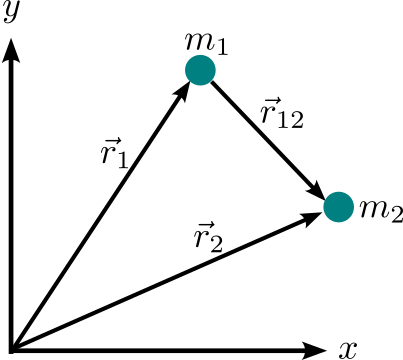
\includegraphics[width=0.35\textwidth]{./two-body.png}
  \caption{A two-body system depicting the gravitational interaction between two particles with masses $m_1$ and $m_2$.} 
  \label{fig:two-body}
\end{figure}

 Since the gravitational force is a symmetric interaction, the force acting on $m_2$ due to $m_1$ is given by
\begin{equation}
  \mathbf{F}_{21} = -\mathbf{F}_{12}
\end{equation}

Therefore, the total force $\mathbf{F}_i$ on body $i$, due to its interactions with the other $N-1$ bodies is obtained by summing all the interactions

\begin{equation}
  m_i \frac{d^2\mathbf{r}_i}{dt^2} = \sum_{j=1,j\neq i}^{N} \mathbf{F}_{ij} = -\sum_{j=1,j\neq i}^{N} \frac{G m_i m_j}{|\mathbf{r}_{ij}|^3} \mathbf{r}_{ij}
\end{equation}
and dividing by $m_i$ both sides we obtain Eq. 1, which describes the acceleration of the $i-th$ body due to the gravitational interactions with the other $N-1$ bodies. For simulation purposes, the denominator $|\mathbf{r}_i - \mathbf{r}_j|$ is usually replaced by  $(|\mathbf{r}_i - \mathbf{r}_j|^2 + \epsilon^2)^{3/2}$---often referred to as the softening parameter $\epsilon$---to avoid singularities when two particles are very close to each other. 

\section{The Barnes-Hut Algorithm}
As previously mentioned, the direct method scales poorly with large systems---and hence---we need to find a more efficient way to compute the forces acting on each body. The Barnes-Hut algorithm is an approximation algorithm for performing an N-body simulation with a time complexity of $\mathcal{O}(N\log N)$. The main idea is to approximate long-range forces by replacing a group of distant bodies with their centre of mass. In exchange for a small loss of precision, this scheme significantly speeds up calculations. It utilises a hierarchical tree structure---a quadtree in 2D and an octree in 3D---to represent the spatial distribution of bodies and their interactions (see Figure \ref{fig:barnes-hut}).

\begin{figure}
  \centering
  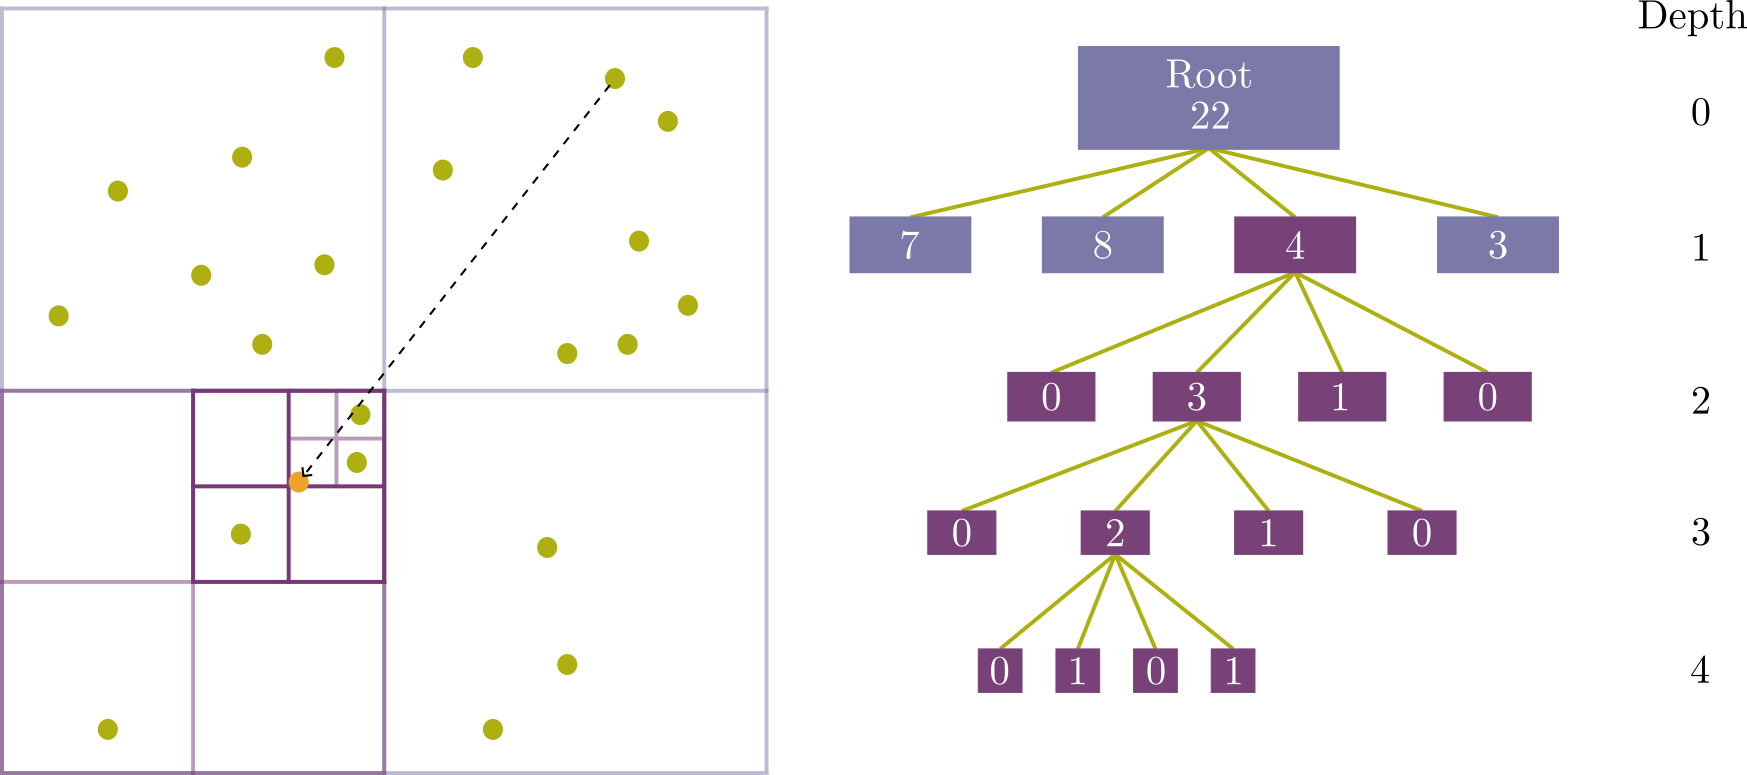
\includegraphics[width=1\textwidth]{./BH-tree.png}
  \caption{A Barnes-Hut tree structure for a two-dimensional system of particles. The root node represents the entire simulation area, and each subsequent level divides the area into quadrants (four child nodes). If sufficiently far away, the node is treated as a single body with mass $M$ and position $\vec{r}_{cm}$ (orange circle).}  
  \label{fig:barnes-hut}
\end{figure}

The tree is built by recursively subdividing the simulation area into quadrants until each node contains either zero or one body---namely a leaf node. We then keep track of the size, total mass and centre of mass for each node, as these will be used to update the state of the system afterwards. These quantities are computed as follows
\begin{equation}
  M = \sum_{i=1}^{n} m_i
\end{equation}
\begin{equation}
  \mathbf{r}_{cm} = \frac{1}{M} \sum_{i=1}^{n} m_i \mathbf{r}_i
\end{equation}
where $n$ is given by the number of bodies in the node. 

Once the tree has been built and the centre of mass and total mass of each node have been updated, we proceed to compute the forces acting on each body. For this, we define a condition---the theta criterion---which determines whether a node is sufficiently far away from the body being considered, such that the approximation is valid. The theta criterion is defined in terms of the size of the node $s$ and the distance $d$ from the body to the centre of mass of the node, $s/d < \theta$. Here, theta is a parameter between 0 and 1 that determines the accuracy of the approximation, and in consequence, the speed of the algorithm. Should the condition be satisfied, the force acting on the body is computed as if the node were a single body with mass $M$ and position $\mathbf{r}_{cm}$ (see Figure \ref{fig:barnes-hut}); otherwise, the algorithm recursively traverses the tree, visiting the child nodes until the condition is met or a leaf node is reached.   


\section{Simulation Setup}
In this section we outline the main components of the implementation of the algorithms. A complete description of the implementation and the source code can be found in the GitHub repository \url{https://github.com/quantum-gabo/N-Body-Simulation}

\subsection{Data Structures}
The implementation of the direct method and the Barnes-Hut approximation requires the definition of some objects and data structures to represent the bodies, 2D vectors and the quadtree. Here below we list and describe the main data structures used in the implementation.
\begin{itemize}
  \item \texttt{Body} class: represents a particle in the simulation. It stores the mass, radius, position, velocity, acceleration, previous position and a boolean flag to indicate if the body is a central body (\emph{e.g.} a black hole).

  \item \texttt{Vector2D} class: represents a two-dimensional vector. It provides methods for vector addition, subtraction, multiplication by a scalar, and computing the norm of the vector. This class is used to represent the position, velocity, and acceleration of bodies in the simulation.

  \item \texttt{Quadtree} class: integrates other two classes---\texttt{Node} and \texttt{Quad}---to represent the tree structure used in the Barnes-Hut algorithm. It provides methods for inserting bodies into the tree, updating the centre of mass and total mass of nodes, and traversing the tree to compute the forces. Once a parent node has been subdivided, its index is added to a vector \texttt{parents}, and the child nodes are stored in a vector \texttt{nodes}.  Each parent node stores the index of its first child node, and each node stores the index of the following node used to guide the traversal of the tree. 
\end{itemize}

\subsection{Initial Conditions and Time Integration}
Equation (4) is a second-order ordinary differential equation (ODE). Since we are working in 2D, the overall system consists of $2N$ second-order ODEs, and hence, require $4N$ initial conditions. These initial conditions include the two Cartesian components of position $\mathbf{r}_i$ and the two components of the velocity $\mathbf{\dot{r}}_i$ of each one of the $N$ particles.

On the other hand, to simulate the system over time, we need to integrate the equations of motion so we can predict the state of the system at time $t+\Delta t$, given its state at time $t$. A variety of numerical integrators can be used, such as Euler, Verlet, or Runge-Kutta. Since we are simulating a physical system with many interacting particles, it is crucial to use a stable integrator. For this reason, we choose Verlet integration, as it is numerically stable, time-reversible, and conservative, making it well-suited for simulations of this nature \cite{book:8675}. The Verlet integration is defined as follows

\begin{equation}
  \mathbf{r}_i(t+\Delta t) = 2\mathbf{r}_i(t) - \mathbf{r}_i(t-\Delta t) + \mathbf{a}_i(t) \Delta t^2 + \mathcal{O}(\Delta t^4)
\end{equation}
where $\mathbf{a}_i(t)$ is the acceleration of the $i$-th body at time $t$ and $\Delta t$ is the time step. Moreover, since Verlet is not a self-starting method, the first step requires the use of a suitable approximation given by
\begin{equation}
  \vec{r}_i(t_1) = \vec{r}_i(t_0) + \vec{v}_i(t_0)\Delta t + \frac{1}{2} \vec{a}_i(t_0) \Delta t^2 + \mathcal{O}(\Delta t^3)
\end{equation}
this allows us to compute the positions of the bodies at the first time step where no previous position is available. Subsequent steps will use Eq. (8) to perform the integration. 

%\subsection{Pseudo-code}
%In this section we provide the pseudo-code for both algorithms, showcasing the main steps and the logic behind the implementation.  
%\begin{algorithm}[H]
%  \caption{\textbf{Direct Method}}
%  \label{alg:brute_force}
%  \begin{algorithmic}[1]
%    \STATE Initialise positions and velocities of the $N$ bodies
%    \STATE Set time step $\Delta t$
%    \WHILE{simulation not finished}
%      \STATE Initialise acceleration $\mathbf{a}_i(t) = 0$ in parallel
%      \FOR{$i=1$ to $N$} 
%        \STATE Compute acceleration $\mathbf{a}_i(t)$ using Equation (4)
%      \ENDFOR
%      \STATE Update positions $\mathbf{r}_i(t+\Delta t)$ in parallel using Verlet integration (Eq. 7)
%    \ENDWHILE
%\end{algorithmic}
%\end{algorithm}

%\begin{algorithm}[H]
%  \caption{\textbf{Barnes-Hut Algorithm}}
%  \label{alg:barnes_hut}
%  \begin{algorithmic}[1]
%    \STATE Initialise positions and velocities of the $N$ bodies
%    \STATE Set time step $\Delta t$
%    \STATE Initialise an empty quadtree
%    \WHILE{simulation not finished}
%      \STATE Clean the quadtree
%      \STATE Initialise acceleration $\mathbf{a}_i(t) = 0$ in parallel.
%      \FOR{$i=1$ to $N$}
%        \STATE Insert body $i$ into the quadtree.
%      \ENDFOR
%      \STATE Update the centre of mass and total mass of each node in the quadtree.
%      \STATE Compute the acceleration $\mathbf{a}_i(t)$ for each body in parallel using the quadtree.
%      \STATE Update positions $\mathbf{r}_i(t+\Delta t)$ in parallel using Verlet integration (Eq. 8).
%    \ENDWHILE
%  \end{algorithmic}
%\end{algorithm}


\section{Results and Discussion}
In this section we present the results of the performance comparison between the direct method and the Barnes-Hut algorithm. Each system size was simulated for 100 time steps, and the execution time of each time step was recorded. Then, the average execution time was computed for each system size. The obtained data is summarised in Table \ref{tab1}, which shows the average execution time for both methods, along with the speedup factor defined as the ratio between the execution time of the direct method and the Barnes-Hut algorithm. Figure \ref{fig:speedup} shows the performance comparison between the two methods, where the execution time is plotted in logarithmic scale against the number of particles.

\begin{table}[h!]
\caption{Execution time for varying system sizes using the direct method and Barnes-Hut approximation, along with the speedup factor.}
\label{tab1}
\begin{tabular}{|l|l|l|l|}
\hline
\textbf{Number of Particles} & \textbf{Direct Method (s)} & \textbf{Barnes-Hut (s)} & \textbf{Speedup} \\
\hline
100     & 0.000048   & 0.000046   & 1.04   \\
500     & 0.000877   & 0.000542   & 1.62   \\
1000    & 0.003328   & 0.001538   & 2.16   \\
2000    & 0.011730   & 0.001769   & 6.63   \\
4000    & 0.054317   & 0.004049   & 13.41  \\
8000    & 0.215674   & 0.009213   & 23.41  \\
10000   & 0.320299   & 0.011732   & 27.29  \\
15000   & 0.734168   & 0.018731   & 39.19  \\
20000   & 1.310772   & 0.025587   & 51.23  \\
30000   & 2.925272   & 0.049420   & 59.18  \\
40000   & 5.189255   & 0.052630   & 98.61  \\
50000   & 8.185188   & 0.069083   & 118.48 \\
60000   & 11.801987  & 0.093106   & 126.75 \\
80000   & 20.728767  & 0.113791   & 182.19 \\
100000  & 32.540323  & 0.152524   & 213.36 \\
\hline
\end{tabular}
\end{table}
\begin{figure}[h!]
\centering
  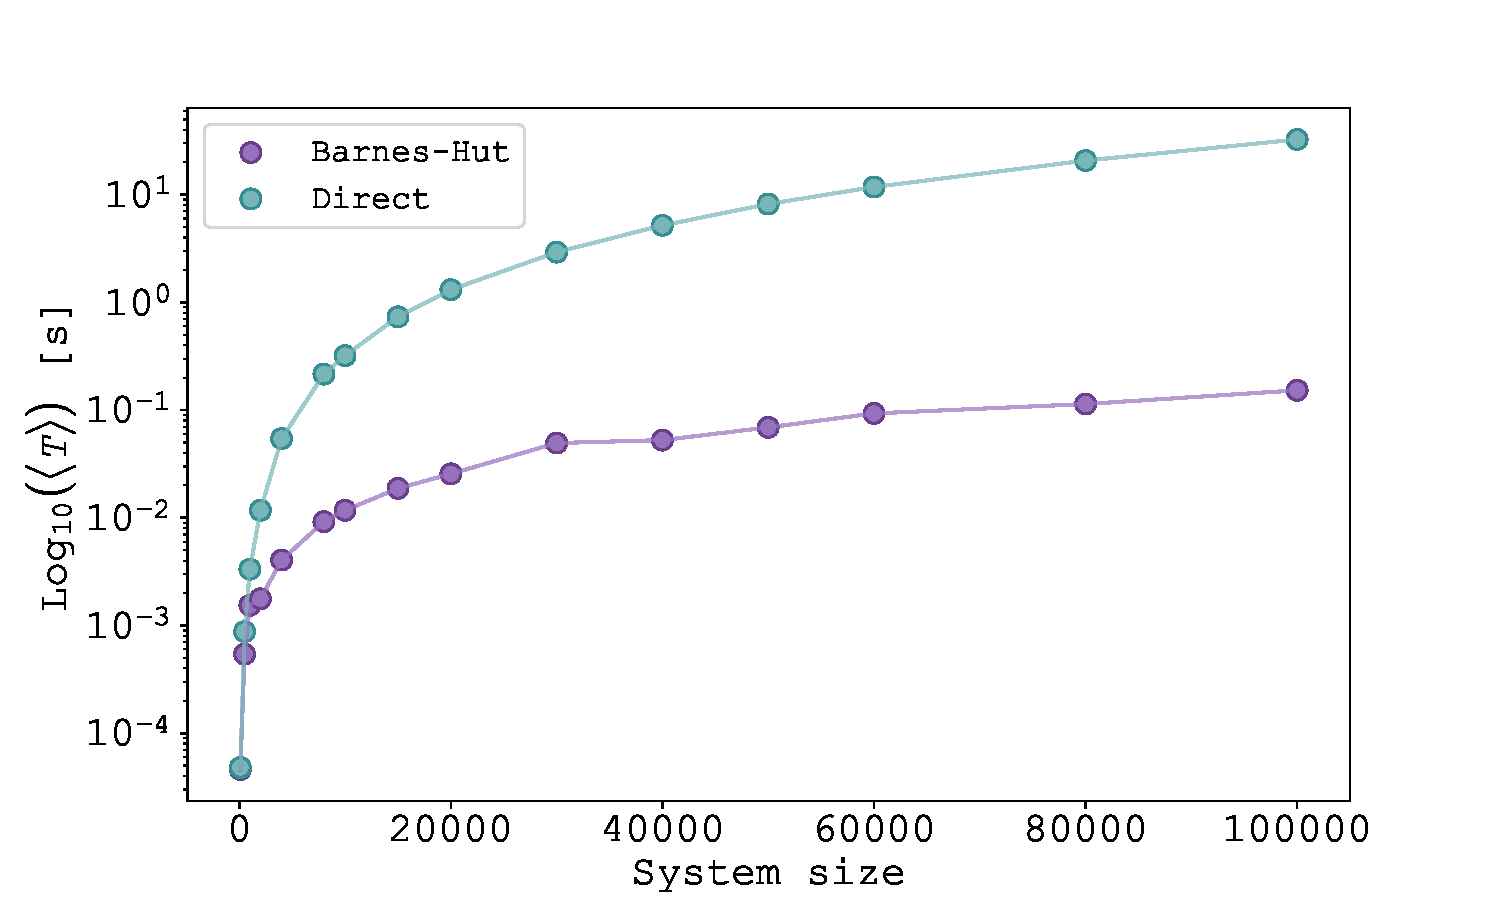
\includegraphics[width=0.8\textwidth]{./benchmark_results.pdf}
  \caption{Performance comparison between the direct method and the Barnes-Hut algorithm. The execution time is plotted in logarithmic scale against the number of particles. The direct method shows a quadratic scaling with the number of particles, while the Barnes-Hut algorithm exhibits a logarithmic scaling.}
  \label{fig:speedup}
\end{figure}

The obtained results show that the direct method and the Barnes-Hut algorithm have a similar performance for small systems---up to $N=500$ particles---where the execution time is in the order of milliseconds. However, as the system size increases, the execution time of the direct method grows rapidly, reaching over 32 seconds for $N=100K$ particles. On the other hand, the Barnes-Hut algorithm maintains a much lower execution time, reaching only 0.15 seconds for the same system size. The speedup factor increases significantly with the number of particles, reaching over 200 for $N=100K$ particles. This demonstrates the effectiveness of the Barnes-Hut algorithm in reducing the computational cost of N-body simulations. Finally, parallel processing was used to speed up key operations, such as acceleration computation, integration, and vector resetting.  

\section{Conclusions}

In this work, we have implemented and compared the performance of the direct method and the Barnes-Hut algorithm for solving the gravitational N-body problem. The former has a time complexity of $\mathcal{O}(N^2)$, while the latter achieves a time complexity of $\mathcal{O}(N\log N)$ by approximating distant forces using a hierarchical tree structure.

The results show that the direct method is suitable for small systems, whereas the Barnes-Hut algorithm outperforms it for larger systems, achieving a significant speedup factor over 200x for $N=100K$ particles. This makes the Barnes-Hut algorithm a more efficient choice for N-body simulations, especially in astrophysical and cosmological applications where large systems are common.
Finally, core components of the implementation were parallelised using the \texttt{OpenMP} library, which further improved the performance of both methods, without adding significant complexity to the code.

%\begin{credits}
%\subsubsection{\ackname} A bold run-in heading in small font size at the end of the paper is
%used for general acknowledgments, for example: This study was funded
%by X (grant number Y).

%\subsubsection{\discintname}
%It is now necessary to declare any competing interests or to specifically
%state that the authors have no competing interests. Please place the
%statement with a bold run-in heading in small font size beneath the
%(optional) acknowledgments\footnote{If EquinOCS, our proceedings submission
%system, is used, then the disclaimer can be provided directly in the system.},
%for example: The authors have no competing interests to declare that are
%relevant to the content of this article. Or: Author A has received research
%grants from Company W. Author B has received a speaker honorarium from
%Company X and owns stock in Company Y. Author C is a member of committee Z.
%\end{credits}
%
% ---- Bibliography ----
%
% BibTeX users should specify bibliography style 'splncs04'.
% References will then be sorted and formatted in the correct style.
%
\bibliographystyle{splncs04}
\bibliography{bibliography}
%
%\begin{thebibliography}{8}
%\bibitem{ref_article1}
%Author, F.: Article title. Journal \textbf{2}(5), 99--110 (2016)

%\bibitem{ref_lncs1}
%Author, F., Author, S.: Title of a proceedings paper. In: Editor,
%F., Editor, S. (eds.) CONFERENCE 2016, LNCS, vol. 9999, pp. 1--13.
%Springer, Heidelberg (2016). \doi{10.10007/1234567890}

%\bibitem{ref_book1}
%Author, F., Author, S., Author, T.: Book title. 2nd edn. Publisher,
%Location (1999)

%\bibitem{ref_proc1}
%Author, A.-B.: Contribution title. In: 9th International Proceedings
%on Proceedings, pp. 1--2. Publisher, Location (2010)

%\bibitem{ref_url1}
%LNCS Homepage, \url{http://www.springer.com/lncs}, last accessed 2023/10/25
%\end{thebibliography}
\end{document}
